%%%%%%%%%%%%%%%%%%%%%%%%%%%%%%%%%%%%%%%%%%%%%%%%%%%%%%%%%%%%%%%%%%%%%%%%%%%%%%%%
%2345678901234567890123456789012345678901234567890123456789012345678901234567890
%        1         2         3         4         5         6         7         8

\documentclass[letterpaper, 10 pt, conference]{ieeeconf}  % Comment this line out
                                                          % if you need a4paper
%\documentclass[a4paper, 10pt, conference]{ieeeconf}      % Use this line for a4
                                                          % paper

\IEEEoverridecommandlockouts                              % This command is only
                                                          % needed if you want to
                                                          % use the \thanks command
\overrideIEEEmargins
% See the \addtolength command later in the file to balance the column lengths
% on the last page of the document

\usepackage[utf8]{inputenc}
\usepackage[T1]{fontenc}
\usepackage{float}
\usepackage{pgfplots}
\pgfplotsset{width=8cm,compat=1.9}
\usepackage{caption}
\usepackage{graphicx}
\usepackage[textwidth=30]{todonotes}
\usepackage{ragged2e}
\usepackage{subfiles}
\graphicspath{ {./Figures/} }


% The following packages can be found on http:\\www.ctan.org
%\usepackage{graphics} % for pdf, bitmapped graphics files
%\usepackage{epsfig} % for postscript graphics files
%\usepackage{mathptmx} % assumes new font selection scheme installed
%\usepackage{mathptmx} % assumes new font selection scheme installed
%\usepackage{amsmath} % assumes amsmath package installed
%\usepackage{amssymb}  % assumes amsmath package installed

\newcommand{\evc}[1]{
\todo[fancyline,color=red!40,size=\scriptsize]{\textbf{ev:} #1
\color{black}}}
\newcommand{\evi}[1]{ \todo[inline,color=red!40]{\textbf{ev:} #1
\color{black}}}



\title{\LARGE \bf
SoK: Classifying Honeypot Fingerprinting Techniques
}

%%%% For Double Blind Version
%\author{Shreyas Srinivasa$^{1}$, Emmanouil Vasilomanolakis$^{2}$, Jens Myrup Pedersen$^{3}$% <-this % stops a space
%\thanks{*This work was not supported by any organization}% <-this % stops a space
%\thanks{$^{1}$S. Srinivasa - PhD Fellow at Department of Electronic Systems,
%        Aalborg University, Copenhagen, Denmark
%        {\tt\small shsr@es.aau.dk}}%
%\thanks{$^{2,3}$E. Vasilomanolakis, J. Pedersen - Asst. Professor at                          Department of Electronic Systems, Aalborg University,                         Copenhagen, Denmark
%        {\tt\small emv@es.aau.dk, jens@es.aau.dk}}%
\begin{document}
\maketitle
\thispagestyle{empty}
\pagestyle{empty}
%%%%%%%%%%%%%%%%%%%%%%%%%%%%%%%%%%%%%%%%%%%%%%%%%%%%%%%%%%%%%%%%%%%%%%%%%%%%%%%%
\begin{abstract}
In defensive security, Honeypots play an important role to detect attacks by simulating the services of the target system. Over the years, many honeypots have been proposed, developed and deployed over the internet simulating essential protocols and services like HTTP, SSH, Telnet, SMB, SMTP, FTP and also industrial protocols like MODBUS and BARCnet. Survey statistics provided by F-Secure \cite{F-Secure}, show that the attack landscape caught by honeypots hosted by F-Secure have tripled from 2018 with major targeted protocols being Telnet, SMB, SSH, and  MSSQL. The rise in attacks can be because of an increase in smart IoT devices and also the accessibility of Cloud infrastructure. Further, resource constraints on IoT devices lead to poor security diligence to achieve performance and availability. Honeypots have been a reliable choice for proactive defense by network administrators to detect and analyze attacks. Open-source low-interaction honeypots like Kippo, Cowrie, Glastopf, Dionaea, and Conpot are the most widely deployed Honeypots \cite{Vetterl2018}. As effective as honeypots can be leveraged to detect attacks, they are also vulnerable to be exposed as decoys thereby reducing their productivity. The identity of honeypots and its ability to remain undetected is a valuable parameter towards its purpose. Studies have shown that these honeypots are easily detectable and can be fingerprint by various mechanisms. Probing, response analysis, and location/domain filtering are some methods through which the identity of honeypots can be revealed. Besides, machine learning-based methods have inferred to increase predictability and reduce false positives in detection. This paper provides an overview and a new basis for the classification of honeypot fingerprinting mechanisms. 
\end{abstract}
%%%%%%%%%%%%%%%%%%%%%%%%%%%%%%%%%%%%%%%%%%%%%%%%%%%%%%%%%%%%%%%%%%%%%%%%%%%%%%%%

%\section{INTRODUCTION}
\section{Introduction}

The rise of the Internet of Things and affordable cloud infrastructure has led to a connected world of devices and services working together to achieve better accessibility and connectivity in real-time. While these devices are resource-constrained, there is more focus on performance and availability rather on security. Also, accessibility being important, leads to various services open to the Internet thereby creating a huge risk in security of the system. Leveraging these known vulnerabilities, proactive security strategies like Honeypots are developed and deployed with these flaws to attract exploits from attackers thereby making them vulnerable by design. Honeypots are classified into three types based on their interaction, service simulation into low, medium and high interaction honeypots. As the name suggests, low interaction honeypots are focused on emulating the basic protocol services and do not focus on high interaction. Low interaction honeypots are quick to set up, highly usable and provide basic logging and analysis features. These honeypots are developed to be deployed in resource constraint environments and perform event logging. Low interaction honeypots are also not security-critical as any damage caused by them as a result of exploitation are minimal.

In addition to various security measures adopted by the administrators, Honeypots form a good defensive tool as decoy systems, to identify vulnerabilities and detect attacks. They act as a proactive approach to identify malicious sources for attacks and also give an understanding of the vulnerable areas of the system. All communication to the honeypot is considered hostile since legitimate users have no obligation to access a honeypot. The use of honeypots as a detection tool date back to over a decade with honeypot projects being open and deployed since the year 2000. Protocols like Telnet and SSH have been widely used even today to establish communication with remote systems. Similarly, protocols like HTTP, FTP, SMTP, SNMP, SMB have been used as base network communication protocols for essential services. There are honeypots developed to emulate all the stated essential protocols. The Honeynet Project \cite{Honeynet} is focused on the development of honeypots for well-known protocols and environments over the years. Administrators have been using these honeypot projects in their DMZ environments to detect the attacks on these protocols over the years. However, it has been evident that these honeypots could be detected and identified. This leads to an argument about the use of outdated honeypots \cite{counting} and their contribution towards attack detection once they are identified.

Honeypot detection is important to notify the developers of these projects of the maintenance. Soon after these projects are released as open-source, very little attention is given to updating or patching. While bad maintenance of any software is a huge security risk, there is also a risk of these projects being deployed more over the world. Once the identity of the honeypots are revealed, their purpose and productivity is degraded. The attackers learn about the honeypot and stay away from engaging any interaction with these systems. Also, honeypots being vulnerable systems by design, form easy entry points for APT exploits from attackers. The main merit of a honeypot is achieved by its ability to remain undetected while continuing interaction with the attacker. It is very important to make sure that this feature is tested by the developers by assuming the role of attackers. Hence, the detection of honeypots provides a good approach to the efficiency of a honeypot. This is very critical especially in the case of low interaction honeypots because of the limited interaction simulations and behavior. There is very less consideration of testing these honeypots before release and deployment. Thus it is crucial and critical for honeypot developers and users to understand these detection mechanisms to make their honeypots more productive and efficient in their deployed environments. A further taxonomy of the fingerprinting methods helps in understanding the resilience of the honeypot. Based on the taxonomy, honeypots can be classified and benchmarked for their resilience. 


Internet-wide scanning has now been convenient and popular because of scanning platforms like Shodan and Censys. These platforms provide search based on region, ports, IP addresses, and domains to check the services vulnerable and open to the Internet. Tools like Nmap \cite{NMap} and Xprobe2 provide good scanning abilities to scan the end systems. Considering Internet-wide scanning as a first step and using the results, it is possible to apply various approaches to determine if the system is a honeypot. We summarize the detection techniques published so far and classify these approaches into Active and Passive approaches of honeypot detection. Further, we use the classification to propose a test suite for honeypots and evaluate various open-source honeypots. However, we also emphasize the fact that all low interaction honeypots can be detected given enough time for replay and analysis. Our primary intention is to classify methods to fingerprinting honeypots based on their interaction overhead. With this paper we contribute with the following:

 \begin{itemize}
    \item Provide an overview of Honeypot Fingerprinting techniques
    \item Classify the fingerprinting techniques based on minimal and advanced interaction. We also propose the idea of active and passive approaches to fingerprinting honeypots
    \item We use the classification techniques proposed to evaluate against popular open-source honeypots and provide remedies to defend against these approaches
 \end{itemize}

%outline of paper
The rest of the paper is structured as follows. Section \ref{sec:back} outlines honeypots and fingerprinting methods.Section \ref{sec:hft} provides an overview of honeypot fingerprinting methods and proposes a taxonomy. In Section \ref{sec:chfm} we classify the detection methods into low and high effort detection systems to further evaluate them in Section \ref{sec:eval} where we evaluate most widely deployed honeypots with the proposed classification. Section \ref{sec:rw} provides an overview of related work done in the honeypot fingerprinting techniques. We finally conclude with Section \ref{sec:conc} by emphasizing the need for new resilient honeypots and new proposed taxonomy for honeypot fingerprinting techniques.

%\section{Background}
\section{Background}
\label{sec:back}

Honeypots are one of the strategies employed in defensive security to detect attacks from adversaries. They are designed and developed to mimic the real protocols and provide information about the attack to the administrators. This section provides an overview on honeypots, detection methods and previous works on fingerprinting techniques. Based on the interaction and service emulation, honeypots are classified into low, medium and high interaction honeypots. Security administrators often feel that low interaction honeypots are feasible to be deployed in their environment as they are not resourced intensively and are less risky. Low interaction honeypots are limited in protocol emulations and hence are also easy targets for fingerprinting attacks. 

Fingerprinting techniques are used to identify systems by analysis of the behavioral information retrieved by probing. It is normally the first step employed by attackers to gain more insight into the end system before exploiting them. This technique has proved to be effective and there are various fingerprinting tools available that can accurately determine the operating system, kernel versions, protocol versions, device name and other attributes of the end system. However, determining these attribute information may involve multiple scans and intermittent probing. The ideal outcome of device fingerprinting infers the device and its attributes, based on which the attacker can orchestrate exploits. The primary focus of a honeypot lies in its ability to stay undetected. Attackers use fingerprinting as an initial setup to determine the validity of the end device before investing their resources on exploitation. If the identity of honeypot is revealed during the initial fingerprinting techniques, their productivity is degraded. This happens due to two reasons. Firstly, the attacker decides to broadcast his findings about the existence of the honeypot which alerts other attackers when they are looking for targets. Second, there is a derived fingerprinting technique for the target honeypot, which can be included in the primary scan of popular fingerprinting tools. p0f, Nmap, Uniscan, Metasploit, Nikto, and cisco-torch are some of the open-source fingerprinting tools which are capable of detecting honeypots like Kippo, Cowrie, and Glastopf. Table \ref{tab:Table1} provides a list of protocols and the honeypots available on the Internet. 

    \begin{figure}
    \begin{center}
    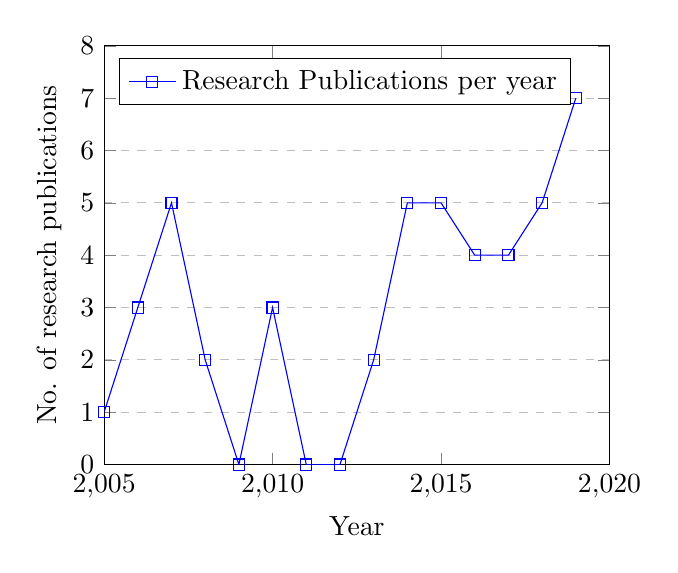
\begin{tikzpicture}
    \begin{axis}[
   %% title={Research on System and Network Fingerprinting},
    xlabel={Year},
    ylabel={No. of research publications},
    xmin=2005, xmax=2020,
    ymin=0, ymax=8,
    xtick={2005,2010,2015,2020},
    ytick={0,1,2,3,4,5,6,7,8},
    legend pos=north west,
    ymajorgrids=true,
    grid style=dashed,
    ]

    \addplot[
    color=blue,
    mark=square,
    ]
    coordinates {
    (2005,1)(2006,3)(2007,5)(2008,2)(2009,0)(2010,3)(2011,0)(2012,0)(2013,2)(2014,5)(2015,5)(2016,4)(2017,4)(2018,5)(2019,7)
    };
    \legend{Research Publications per year}
    
    \end{axis}
    \end{tikzpicture}
    \end{center}
    \caption{Research on System and Network Fingerprinting}
    \label{fig:research_per_year}
   \end{figure} 
    

Identifying deviations in the behavior of a system and inferring fingerprints has been an active research topic. Early works by Brumley et al.  involved a theoretical approach based on the binary analysis \cite{Brumley}. All attacks towards honeypots are recorded or logged for further analysis. This process is an expensive operation considering the writes and file operations thereby creating a delay in the response times of the honeypot. Further, honeypots utilize virtual environments to save resources in their environment. Based on these ideas, Holz et al  proposed that honeypots could be detected due to an increase in the execution time of the commands from the attackers because of logging and sandboxing \cite{Holz}. Fu et al.  also, suggested that the delay in execution and the response due to the virtualized network layer leveraged by honeypots could be a factor to infer the presence of the honeypot \cite{Fu}. At the Black Hat conference 2015, Cymmetria research  proposed various factors by which honeypots could be fingerprinted and recommended new design strategies and development practices to overcome the detection \cite{BLACKHAT}. Alexander et al.  provide a systematic fingerprinting approach for low-interaction honeypots \cite{Vetterl2018}. They leverage the faults of poorly maintained libraries referenced in the emulation of protocols in popular honeypots. The libraries used in the development of protocols in honeypots were not intended to reproduce the actual behavior of the protocol itself but used for the ease of development. The authors present a fingerprinting approach by the development of probes that trigger the response at the transport layer and were successful in identifying up to 7605 honeypots online. Their research is limited to SSH, Telnet, and HTTP honeypots. Internet scanning tools like Shodan have also released Honeypot identification methods called Honeyscore \cite{SHODAN}. The tool accepts an IP address or a URL as an input and provides a result if the end system is a honeypot. The tool is stated to be still in development but is capable of recognizing popular honeypots on the Internet. Feng et al.  propose a machine learning model to collect and classify the response data received from \acrlong{ics} open on the Internet \cite{Feng2016}. The approach relies on the flawed implementation of industrial control protocols and the deployment configurations of the honeypots. Figure \ref{fig:research_per_year} shows the increasing research in the area of system fingerprinting over the years. Over the last five years, there is a consistent increase in fingerprinting research techniques. This rise in fingerprinting research shows that there are significant methods that can detect end systems. Classification of these methods and proposing a taxonomy enables better analysis and development of resilient systems. 



\begin{table*}[ht!]
\caption{\label{tab:Table1}Protocols and Honeypots}
\centering
 \begin{tabular}{||c c c c c c c||} 
 \hline
 SSH & Telnet & HTTP & SMB & Database & \acrshort{ics} & IoT\\ [0.5ex] 
 \hline
 Kippo & Telnet-IOT-Honeypot & Dionaea & HoneySMB & mysql-honeypotd & Conpot & HoneyThing\\ 
 
 HosTaGe &  HosTaGe &  HosTaGe &  HosTaGe &  HosTaGe &  HosTaGe &  HosTaGe  \\
 
 Cowrie & Cowrie & Glastopf &  & pghoney & GasPot & Kako\\

 Blacknet & TPwd & Conpot &  & MongoDB-HoneyProxy & GridPot & IotPot\\
 
 Kojoney2 & MTPot & Nodepot & & & & \\
 
 MockSSH & Hontel &  &  & & & \\ [1ex] 
 \hline
\end{tabular}

\end{table*}


\section{Honeypot Fingerprinting Techniques}
\label{sec:hft}

%We now present various fingerprinting techniques for honeypots. The techniques are inferred from related work in the area of fingerprinting and contributions from researchers. Based on their type, we list four methods for fingerprinting of honeypots. Figure \ref{fig:taxonomy} summarizes the honeypot fingerprinting techniques. The taxonomy provides an overview of fingerprinting techniques and classifies them based on the approach. The techniques are further classified based on the detection and interaction models. The proposed taxonomy provides insights into efforts required for the determination of the honeypots. We classify the detection models .


Based on the background of fingerprinting research, we propose a taxonomy for honeypot fingerprinting. 
We propose a two tier taxonomy. The first tier classifies the fingerprinting techniques based on the detection methods.The second tier classifies the fingerprinting methods based on their interaction with the honeypots.
Tier 1 provides a top level outline of the honeypot fingerprinting techniques based on the detection scope. We principally classify them into Meta-data based, Probe based, Dependency based and Machine Learning Based techniques. Tier 2 further extends the classified techniques in Tier 1 to distinguish them into low and high effort techniques based on their interaction with the honeypots. This 2-Tier taxonomy provides an characteristic overview of the honeypot fingerprinting techniques. Figure \ref{fig:taxonomy} provides an overview of the Taxonomy based on Tier 1 and Tier 2. The rectangles represent Tier 1 and the squares represent Tier 2. We describe the tier based classifications in the below sub sections. 


\subsection{Meta-Data based fingerprinting}
Metadata based fingerprinting leverages the basic known information about the honeypot. This method is  not dependent on any interaction with the honeypot to determine any information. The technique utilizes basic information like the IP address or the domain name to infer the probability of honeypot existence. With IP address information, it is possible to determine other metadata about the system like the geo-location, \acrshort{isp}, \acrshort{as}, hosting or cloud provider. This metadata can be further analyzed to determine the probabilities of a honeypot. For example, if the target system has the \acrshort{tcp} port 500 open and the IP address is geo-located to assigned to an University, it can be possible that the target system is a research honeypot. Another example would be if the same system is found to be hosted by a cloud provider like \acrshort{aws}, the system is likely a honeypot because Industrial Control Systems are physical devices that cannot be hosted or deployed on a cloud infrastructure.

\begin{figure}[t]
    \centering
    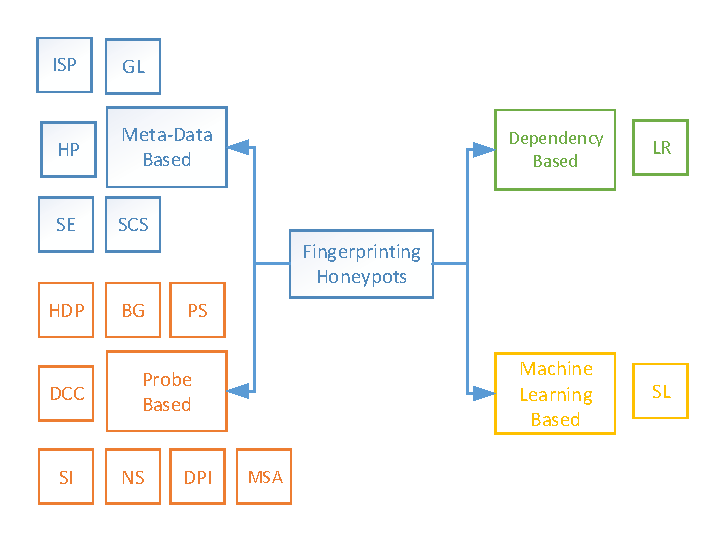
\includegraphics[scale=0.7]{taxonomy2}
    \caption{Honeypot Fingerprinting Taxonomy}
    \label{fig:taxonomy}
\end{figure}


Internet-wide scanning tools like Shodan provide honeypot detection services. Shodan uses active probing techniques and list the services active on the target systems. Shodan's  HoneyScore service accepts either an IP address or a URL to check in its database and provides feedback if the target system is a honeypot. Shodan describes that the service works by using the characteristics of known honeypots and assigning a score from 0.0 to 1.0 based on a match of the characteristics. The scores are stored in a native database. The service is still under development but is capable of detecting popular honeypots listed in Table \ref{tab:Table1}. Shodan also provides an API that can be used to integrate in scanning or fingerprinting scripts. The information collected by Shodan can be leveraged to determine the services running on the target system without interacting with the actual system. In addition, Shodan provides other essential metadata like HTTP content, response parameters, certificates and other technical parameters that can be used for fingerprinting. Other metadata-based fingerprinting methods include using search engines to collect information about the target system. Popular search engines crawl through the Internet daily to improve search results. With the search information, it is possible to identify and group relevant information to determine additional facts for the fingerprinting approach. 

Based on the information received from meta-data methods, it is possible to infer the existence of a honeypot with minimal interaction. We formulate the process of fingerprinting with the metadata approach based on the data received through the process. The parameters like geo-location provide information about the location of the honeypot. This information can be used to find relevance to the services rendered by the honeypot. For example, if the location is identified as an educational institution, the system is likely a honeypot deployed for experimental purposes. Similar inferences can be made with the data received from other parameters like ISP and hosting information. In the following subsections, we provide further information about the information that can be derived using metadata. 

\subsubsection{Geo-Location(GL)}
The location of a system determines what sector it is being used. It is possible to accurately determine the location of any system bearing a public IP address. This information is particularly useful when the system is suspected to be in a location that is not relevant to the services it is offering. This information can be used to derive that the target is either a training system or a honeypot. 

\subsubsection{\acrfull{isp}}
With the IP address information, it is possible to find the \acrshort{isp} that the address pool belongs to. This is especially useful in deriving information about the service providers to industries and corporate environments. Normally, enterprises have dedicated leased lines or fiber lines from well-known service providers. Also, service providers may deploy many honeypots in their management networks as a proactive defense strategy. For example, if the IP address is assigned to a hosting service like \acrshort{aws}, the \acrshort{isp} is listed as Amazon. This information can be used to infer that the system is a honeypot as Amazon is not a generic \acrshort{isp}. 

\subsubsection{Hosting Provider(HP)}
The hosting of the target system is good evidence of the implication of a honeypot. If the target is found to be hosted with a cloud provider, with pointless services, it is very conclusive that the target is a honeypot. Also, if the system is hosted with an unrelated domain pool that differs from the content of the honeypot, it can further lead to the inference of being a honeypot. It is very important for honeypot developers to create content and responses that relate to the hosting domain. 

\subsubsection{Social Engineering(SE)}
Social Engineering is a leading Offensive Security strategy. Most of the findings from other attackers are documented or reported on fingerprinting databases. Social engineering through Internet search engines can provide meta-data about honeypot signatures and fingerprinting information. Searching the metadata with sensible parameters on an advanced Internet search engine can provide interesting information about the target system. This information may include the past activity with the system, exploits, findings which can be used to infer that the target is a honeypot. The source of the information can be used in a scan script as a search database for fingerprinting. 

\subsubsection{Shodan/Censys Search (SCS)}
Shodan is a database of vulnerable systems on the Internet. It provides search as a service by accepting IP address, hostname or service names as search parameters. The output contains information about the target system and its open services. Shodan also provides a Honeypot Detection service called HoneyScore  in addition to the database of vulnerable systems \cite{SHODAN}. Shodan performs daily scans of the Internet with probe-based fingerprinting methods to identify vulnerable systems on the Internet. It has also a major source for attackers to get fast access to vulnerable systems. Though Shodan and Censys use active probing to detect and collect technical information about the target systems, we leverage the information stored in their repositories as metadata to determine if the target system is a honeypot. Similarly, Censys provides advanced querying of the data collected from the internet wide scan. 

Censys is another Internet-wide search engine that is similar to Shodan. It makes use of the ZGRAB  utility to collect application-level data of the services running on the target machine \cite{censys}. Censys also offers a query-able search based on the specific service running on the target system. Censys performs daily Internet-wide scans and aggregates the data in a query-able database. It differs from Shodan by providing a query-based search towards application-level data. Censys does not provide a honeypot detection service yet. Both Shodan and Censys provide reporting capabilities and offer API's. 

\subsection{Probe based fingerprinting}
\label{Probe Based}
Probe-based fingerprinting involves the creation of crafted queries to target devices to derive fingerprinting information. The probe-based methods engage with the target system, unlike the metadata methods. These methods focus on leveraging the responses from communication protocols and classifying the target machine based on specific values from the responses. Constructing probes is an advanced method that requires proficient knowledge of systems and protocols. Therefore extensive knowledge about systems and protocols is necessary for probe-based methods. The queries are constructed to trigger specific information from the target machine. The information may include system-specific unique values for parameters like \acrfull{icw} or \acrfull{rto}. 

Shu et al.  proposed the fingerprinting of network protocols with a formal approach \cite{shu2006network}. The approach proposes a \acrfull{pefsm} to formally model protocol specification and candidate conforming implementations. Several fingerprinting tools like NMap, Metasploit and Hydra make use probe-based methods to determine the operating systems and the protocol versions of the target systems. These tools rely on TCP packet information to determine the operating system. The specific values unique to each operating system are logged in the database of the tool. This helps in comparison to the value of parameters obtained by probing and determine the operating system by matching the closed parameter value from the database. We discuss different probe-based techniques in the following.

\subsubsection{Port Scanning(PS)}
Port scanning is the a technique to determine the open ports and services on the target system. It forms the first step before attacking a target system. Port scanning involves scanning and listing open ports on the target system. Ports that are open signify that they are open for communication and the active services on the system. Many administrators leave the services running on default ports and configuration. For example, port 22 is used for SSH and port 80 for HTTP web service. Port scanning provides information about the transport layer protocol used, the port number and the status of the port. Popular port scanning tools like NMap provide more information about the open ports like the active service, version and the vulnerabilities associated with the version \cite{NMap}. NMap also provides fast scans and detailed scans that recognizes six port states and classifies them into open, closed, filtered, unfiltered, open-filtered and closed-filtered. It has a database of fingerprinting information for 2000 services. 
Tools like NMap and ZMap provide parameterized scripts to run port scanning on target machines \cite{zmap}. Furthermore, custom scripts have been developed with NMap that can identify honeypots like Kippo and Dionaea.  

\subsubsection{Banner Grabbing(BG)}
Banner grabbing is one of the techniques used in the reconnaissance process following a port scan. After learning about the open ports, a connection is established with the remote system to get information about the service and the version number. Some implementations of protocols like FTP and HTTP expose critical system information like service name, software, version, and the operating system. Banner grabbing based probes targeted on a protocol can reveal vulnerabilities associated with any critical information obtained. The CVE database provides a list of vulnerabilities associated with protocols, software and operating systems  \cite{CVE}. Popular tools for Banner Grabbing are Wget\cite{wget}, cURL\cite{curl}, NMap\cite{NMap}, Netcat\cite{netcat}, and Dmitry\cite{dmitry}. Banner grabbing can be used not only for netfork fingerprinting, but also for application fingerprinting. Damron et. al  demonstrates that banner grabbing can be effectively used to fingerprint application software through requests \cite{bannergrab}. The author considers Apache Web Server as an example and presents distinct response codes from the banner that can be used fingerprinting. Alexander et. al  show that banner response from honeypots like Kippo showcase distinct values that can be used for fingerprinting the honeypot \cite{Vetterl2018}. Censys also provides a feature for querying the database with specific values in the banner response. Banner grabbing is also an integrated feature with port scanning on most of the port scanning tools. 

\subsubsection{Handshake Proposals(HSP)}
TLS handshake is a protocol process that establishes the parameters for secure communication between systems. The handshake process involves the exchange of messages to acknowledge each other, the TLS version,  negotiate the cipher suites, authentication with the public key and session keys generation. Besides, there are parameters like message size and timestamp. TLS negotiations are transmitted in plaintext. With the information available through this negotiation, it is possible to fingerprint the client and server applications.  The handshakes also determine the cipher suites proposed by the target system. This information can be leveraged to find vulnerabilities and to characterize the systems based on limited choice of ciphers. The handshake process provides information about the server system that can be used for fingerprinting. As many honeypots depend on static libraries, careful comparison of the actual and the target system responses can reveal if the target system is a honeypot. 
JA3 and JA3s are techniques developed that can actively fingerprint the TLS client and servers based on their hello messages \cite{JA3}. 



\subsubsection{\acrfull{dpi}}
\acrfull{dpi}  is a method for analyzing and monitoring network traffic. Using DPI, network packets can be filtered based on the protocol type and the data in packet components. Conventional packet inspection methods examine only the header information for filtering the traffic. DPI is performed at enterprises using layer 6 devices like firewalls or intrusion detection systems. DPI can help to identify redundant responses received from a machine for fingerprinting purposes. DPI relies on a repository of existing protocol fingerprints for classification. It is an effective technique used by IDS to filter malicious packets from the production networks. On the contrary, DPI can be an effective technique to fingerprint honeypots or protocols based on the header and the payload information. Sang et al. proposed a fingerprinting technique based on byte embedding for the classification of network protocols \cite{Sang}. The approach learns the application fingerprints from traffic traces by characterizing the packet payloads with a byte embedding based payload alignment algorithm. However, with open-source libraries and tools like nDPI, it is possible to fingerprint and inspect various protocol services on the honeypot \cite{nDPI}. DPI requires good knowledge of packet-level communication and networking. It is an advanced probe-based method that requires advanced knowledge for the creation of probes to retrieve specific information from the target system.  


\begin{table}
\begin{tabular}{||c c c c c||} 
 \hline
 Honeypot & Protocol & Language & Library & Updated \\ [0.5ex] 
 \hline
 Kippo  & SSH    & Python &  TwistedConch & May2015 \\ 
 Cowrie & SSH    & Python &  TwistedConch & May2018 \\
 TPwD   & Telnet & C      &  custom       & Feb2016 \\
 MTPoT  & Telnet & Python &  telnetsrv    & Mar2017 \\
 TIoT   & Telnet & Python &  custom       & May2017 \\
 Cowrie & Telnet & Python &  TwistedConch & May2018 \\
 Dionaea& HTTP   & Python &  custom       & Sep2016 \\
 Glastof& HTTP   & Python &  BaseHTTPServer& Oct2016 \\
 Conpot & HTTP   & Python &  BaseHTTPServer& Mar2018 \\ [1ex] 
 \hline
\end{tabular}
\caption{Library references in honeypots}
\label{library}
\end{table}



\subsubsection{Default Configuration Check(DCC)}
Applications are setup with setup scripts or by using install media. Often, these media do not prompt the user to change the default settings or configuration before the final installation. This leaves the system running with a default configuration. For example, we have Apache Tomcat Manager instance running on a default installation of Apache Tomcat. The manager provides an interface to manage the web service and the deployments. It is important to configure the tomcat manager or disable if not used. Similarly, devices and applications are running with default configurations on the Internet. With these default configurations, it is easily possible to fingerprint the target system. Honeypots like Kippo, Cowrie, Glastopf, and Conpot are usually deployed with default configurations. Morishita et al.  provides an approach to self-revealing honeypots on the Internet by detection through default configurations \cite{morishita}.  This leads to the easy discovery of honeypots by constructing a probe to check the default configuration. If the response matches the defaults, the end systems is likely a honeypot.

\subsubsection{System information(SI)}
Systems often reveal or allow to be queried about specific information like the processor family, architecture, network interface and timezone. This specific information help in the inference of a honeypot system. They are useful metadata when combined with data collected from other techniques.  Also, ping response times can be used to detect the operating system of the target system. Early works from Mukkamala et al.  show the detection of low-interaction honeypots and virtual environments based on support vector machine models \cite{mukkamala}. The approach compares the average time taken for responses from a virtual machine than that of a real system. The authors determine the existence of a honeypot by testing the limitations of the services emulated by the honeypot, timing analysis of the ICMP echo requests and TCP/IP fingerprinting with 49 featured data set.  
\newline
\subsubsection{Network Sniffing(NS)}
Network Sniffing is a reconnaissance method used for analyzing the network traffic exchanged between two entities. The traffic is monitored to find anomalies. Any deviation from regular behavior, such as redundant network traffic, broadcasts and logging are easy signs of a honeypot . Sniffing techniques work well if the packet sniffing tools are installed within the same network as a honeypot\evc{I don't get these 2 sentences}. These techniques are also effective to determine the existence of high-interaction honeypots\evc{how?}. However, sniffing methods are ineffective if the attacker is unable to filter packets from the source system. Attackers can still use sniffing techniques if they gain successful access to a vulnerable system. The attackers can install bots to tap the network traffic and have them report to a \acrshort{cac}  server. This can expose other systems in the network of the honeypot. \evc{paragraph not very clear}

\subsubsection{\acrfull{msa}}
\acrlong{msa} can be defined as a sequential array of exploits by an attacker targeting multiple vulnerable services on a system. \acrshort{msa} leverage the vulnerable service on the system to exploit the other services on the same system by gaining more control over the system. These kinds of attacks are key to detection as they help in inferring a relationship between multiple services running on the system that constitutes an environment. Vasilomanolakis et al. proposed a honeypot capable of identifying multi-stage attacks  \cite{vasilomanolakis}. The honeypot is capable of simulating environments by running related services. The honeypot effectively captures advanced persistent threats. However, the information about services running on a system can also infer that the system is not real. For example, in the case of \acrshort{ics}, the communication protocols are active on specific devices and not on a single device. Honeypots like Conpot that are based on \acrshort{ics} show that all the services are running on the target machine. Hence, it can be easily inferred that the target system is a honeypot. 

% will be added in countermeasures 
%\subsubsection{Risks in Probe-Based Fingerprinting}
%\evc{how is this paragraph relevant compared to the previous ones?}
%However, there are risks involved in probe-based fingerprinting methods. As these methods involve direct interaction with the target system, eventually the probe system is blacklisted. We must remember that there is no real reason for establishing a connection with a honeypot. Any connections observed with a honeypot is considered potentially an attack. Probing systems may get blocked by this approach. This limits in further exploitation or identification of the attacker or the honeypot. It is important to keep the attacker engaged with the honeypot to collect as much possible to identify the attacker. 

\subsection{Dependency-based fingerprinting}
Honeypots simulate network protocols. The simulations are usually implemented using pre-built language-specific libraries of protocols that are open-source \cite{Vetterl2018}. Many of the referenced libraries are very old and not maintained. Developers often reference libraries in their project to save time building the library themselves. These libraries are not developed to fully emulate network protocols. They offer basic communication features with some hardcoded response strings. Popular open-source honeypots binaries are available on the Internet. By carefully observing the source code, or the referenced libraries, it is possible to create probes that trigger the static response from the referenced library. For example, the Twisted Conch  library is the most referenced library for SSH protocol simulations in honeypot implementations\cite{twisted}  \cite{counting} . Though there have been recent contributions to the library, there is no change or update made on the honeypots referencing it. Since the library is available as open-source, it can be analyzed for its simulations and static responses can be detected for specially developed probes. The Twisted Conch library also includes simulation for the Telnet protocol. Dependency based detection is an effective method for detecting honeypots based on SSH, HTTP, Telnet, FTP, and Modbus protocols because of their dependency to static libraries. Many honeypots refer to static libraries and this causes static response for carefully crafted requests.There are limited libraries available for the simulation of the above protocols. The honeypots are not updated and still use static responses emulated by the libraries. Table \ref{library}  shows the list of libraries referenced by popular honeypots, protocols, and their versions \cite{Vetterl2018}. 



\subsection{\acrfull{ml} based fingerprinting}
\acrfull{ml} techniques are based on the response data received from probe-based methods. The collection of response data acts as a learning dataset for designing a model for the detection of honeypots. The \acrshort{ml} models depend on data and modeling algorithms to learn the process of fingerprinting based on previous inference in the data set. Huang et al.  provide an \acrshort{ml}-based model approach to detect honeypots\cite{huang}. The approach introduces features from the network layer, application layer, and the operating system layer and proposes a detection model to identify honeypots with a stated detection rate of 0.03 AUC. Feng et al.  also propose a learning model based on the probe-based method for detecting \acrshort{ics} honeypots \cite{Feng2016}. The proposed method initially uses reconnaissance to identify systems open to the Internet with specific ports open which are related to \acrshort{ics}. Next, they construct probes to collect data for specific banners and handshakes. This information is used to design a learning model to classify real systems and honeypots of \acrshort{ics} devices.

\acrshort{ml}-based fingerprinting is recommended when there is enough data to train the supervised learning process. With good learning models and data, it is possible to increase the detection accuracy. This technique is suitable to be applied after successful fingerprinting methods are established for a honeypot through metadata and probe-based fingerprinting techniques. Supervised learning relies on good training data set for its classification. The training data set must be relevant for incorporating new features. The main drawback of this approach is the freshness of the data. The data on which the models are based need to be constantly changed and tested to ensure that the detection accuracy is still maintained. Unsupervised learning techniques can be applicable in such situations. 


\section{Classifying Honeypot Fingerprinting Methods}
\label{sec:chfm}

Traditionally, fingerprinting methods are classified into active and passive based on interaction with the target system \cite{spitzner}. Active fingerprinting involves the creation of specific probes and using them to query the target system to collect as much data possible. On the contrary, passive fingerprinting makes use of available metadata and analysis to determine information about the target. Passive fingerprinting limits communication with the target system as much as possible. Remote attackers tend to use active fingerprinting methods more because passive approaches do not lead to an inference. This is because passive fingerprinting requires detailed analysis of collected meta data. Passive fingerprinting techniques also depend on fingerprint databases to infer their findings. Fingerprint databases contain information about distinct responses by systems on interaction.
   
We further classify the detection methods discussed in sections before into \acrfull{lef} and \acrfull{hef} methods. The classification is based on the communication levels required by the methods to obtain qualified information to fingerprint the target system. Honeypot networks block communication with the attackers after a connection attempt is detected. This limits the detection and further exploitation of the honeypot from a probe network. Also, we believe that \acrshort{lef} methods are effective with honeypots fingerprinting, to limit logging information of the attacker and to avoid being blocked. 

 \subsection{\acrfull{lef}}
 \acrfull{lef} aims at the detection of honeypots with minimal or no direct interaction with the target system. They use metadata-based techniques to fingerprint honeypots. It is necessary to correlate the information obtained from these methods to achieve conclusive results on fingerprinting. This reconnaissance technique is complex because it requires substantial time from the attacker to collect and integrate the metadata to infer the existence of a honeypot. The advantage of using \acrshort{lef} methods for fingerprinting is that the attacker's information remains hidden and no backtracking is possible. These techniques do not require deep knowledge of fingerprinting. The techniques focus on gathering metadata utilizing social engineering methods. While low-effort techniques rely on metadata obtained from the open sources on the Internet, they are advantageous in finding data leaks in an enterprise. 
 
 
 \subsection{\acrfull{hef}}
\acrfull{hef} employ probe-based techniques to interact with the target system to obtain specific operational information from the target system. They leave a massive footprint on the target machine during the probing process. This footprint enables honeypot administrators to trace the attackers or blacklist the IP addresses of attack sources. Though maximal interaction techniques provide better data for detection accuracy, they are risky. Internet-wide scan result providers like Shodan and Censys use \acrshort{hef} techniques to scan the Internet for open ports and vulnerable services. Information from these search engines are used as reconnaissance for exploits. We emphasize that all honeypots are prone to detection over a period of interaction. Accurate fingerprinting data can be obtained by a detailed intelligent scan from probes. \acrshort{hef} methods have detection accuracy as an advantage but are highly susceptible to backtracking. 
   

\section{Evaluation}
\label{sec:eval}

In this section, we evaluate the methods in the proposed taxonomy. The evaluation setup and evaluation process are described in the following sub sections. 

\subsection{Evaluation Setup}
We evaluate the Probe based and the Metadata based methods in our evaluation. For the probe based methods, we create probes for the techniques and scan the Internet. The probes are created using ZMap \cite{zmap}. We limit the \acrshort{ip} address range to Germany to reduce the Internet scanning overhead. The system used for evaluation has a Linux distribution and has a private \acrshort{ip} address allocated by University DHCP server.  The results of the scanning are are not shared publicly. The aim of this evaluation is to detect honeypots based on the proposed taxonomy. The Internet scan is performed for research purposes only. The metadata-based techniques require search keywords to retrieve information about the honeypots. The keywords list is determined using information from publications based on honeypot fingerprinting research \cite{Vetterl2018} \cite{counting}. Furthermore, we determine additional keywords by setting up popular honeypots listed in Table \ref{tab:protocols-honeypots} on our local environments and probing them for static content. The experiment is carried out for a period of one week. 

\subsubsection{\acrshort{fsm} for Probe-based Methods}


\subsubsection{\acrshort{fsm} for Metadata-based Methods}
\label{sec:metadata_fsm}
The \acrshort{fsm} is constructed based on metadata-based fingerprinting methods listed in Figure\ref{fig:taxonomy}. We explain the \acrshort{fsm} created for honeypot fingerprinting in this section. Figure \ref{fig:fsm_md} shows the \acrshort{fsm} created for evaluation of metadata-based methods. The \acrshort{fsm} consists of multiple states with transitions. The states are denoted by the rectangle boxes and the arrows between the boxes denote the transitions. The solid sphere indicates the start state. The green and the red spheres indicate the final states. The numbers zero and one represent true and false. If the metadata based methods were successfully able to extract metadata that can be used for honeypot fingerprinting, we represent the transition as true. If there was no metadata inferred we denote the transition as false. 

We explain the states and the transitions in the \acrshort{fsm} as follows. We begin the process by scanning Shodan and Censys for vulnerable systems exposed to the Internet with SSH, HTTP, MODBUS and Telnet services. The information retrieved from the scan engines is compiled to fingerprint honeypots.With the \acrshort{ip} address of the systems, we can successfully derive the \acrshort{fqdn},Geo-location, hosting provider, \acrshort{isp} of the target system. We use this information in the following states to determine the existence of a honeypot. However, if the metadata is not sufficient to fingerprint, we use this data effectively in the Probe-based methods. 

\begin{figure}[ht]
    \centering
    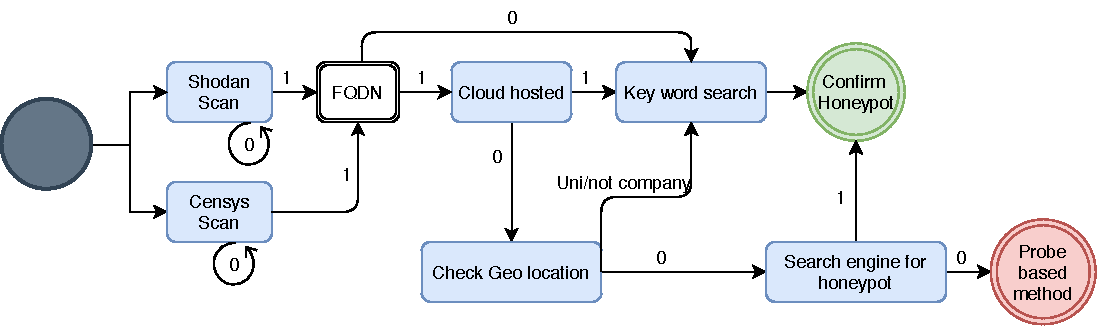
\includegraphics[scale=0.45]{Metadata_FSM}
    \caption{\acrshort{fsm} for Metadata-based Fingerprinting }
    \label{fig:fsm_md}
\end{figure}


\subsection{Evaluation - Probe-based Techniques}
Probe-based techniques require creation of probes to retrieve specific information from the target system. The probes are constructed based on the techniques Probe-based methods depicted in Figure\ref{fig:taxonomy}. We evaluate the methods by developing a fingerprinting tool based on an \acrfull{fsm} model. The \acrshort{fsm} provides a formal approach to the probing process and the aggregation of data received for honeypot fingerprinting. The \acrshort{fsm} for the probe-based techniques is shown in Figurexxx. 


\subsection{Evaluation - Metadata-based Techniques}
Metadata-based techniques leverage the data that is collected without direct interaction with the honeypot. By implementing crawler described in Section \ref{sec:metadata_fsm} we try to fingerprint honeypots on the Internet. We were successfully able to detect and fingerprint around xxx honeypots. The results are summarized in Table xxx.  


 
 
\documentclass[../main.tex]{subfiles}
\begin{document}

\end{document}
 
\section{Related Work}
\label{sec:rw}

Joni et al. \cite{Joni} provides a  summary of research on anti-honeypot methods and propose a taxonomy, based on detection vectors. They classify the detection vectors based on temporal, operational, hardware and environment of the target system. The authors provide informative methods used by malware botnets for detecting honeypots. However, there is no evaluation of the detection vectors in the proposed taxonomy. The future work proposes the development of a honeypot system with dual interface support. The dual interfaces enable a user and software to use the primary interface as a normal system and the secondary interface as a fake system. The secondary interface acts as a honeypot and any interaction raises an alarm. The authors also propose self-aware and dynamic honeypots that adapt and recover from any recognized fingerprinting methods. The proposed taxonomy attempts to consider attacks from an automated botnet malware and does not consider a human-driven attack vector. In 2004, Krawetz et al. \cite{krawetz2004anti} proposed anti-honeypot technology that identifies potential honeypots that capture mail spammers and web servers. The technology aims at using fingerprinting methods that exploit the limited simulation of systems. The author warns that there can be more effective honeypot detection methods evolving in the future that are more accurate. The author provides no taxonomy of these methods. 
 
 
\section{Conclusion}
\label{sec:conc}

Honeypots have been an important strategy in proactive defense systems. They are effective security systems capable of detecting new threat vectors. Honeypots are victims of malware botnets and fingerprinting networks that intend to expose their identities.  We survey and summarize honeypot fingerprinting methods and propose a taxonomy. We evaluate the classified fingerprinting methods against popular honeypots and determine their resilience. As future work, we aim to continue finding new honeypot fingerprinting methods. We further use the new findings and this taxonomy to propose new design considerations for the development of resilient honeypots. 


\addtolength{\textheight}{-12cm}   % This command serves to balance the column lengths
                                  % on the last page of the document manually. It shortens
                                  % the textheight of the last page by a suitable amount.
                                  % This command does not take effect until the next page
                                  % so it should come on the page before the last. Make
                                  % sure that you do not shorten the textheight too much.

%%%%%%%%%%%%%%%%%%%%%%%%%%%%%%%%%%%%%%%%%%%%%%%%%%%%%%%%%%%%%%%%%%%%%%%%%%%%%%%%
%%%%%%%%%%%%%%%%%%%%%%%%%%%%%%%%%%%%%%%%%%%%%%%%%%%%%%%%%%%%%%%%%%%%%%%%%%%%%%%%
%%%%%%%%%%%%%%%%%%%%%%%%%%%%%%%%%%%%%%%%%%%%%%%%%%%%%%%%%%%%%%%%%%%%%%%%%%%%%%%%
\section*{ACKNOWLEDGMENT}
%%%%%%%%%%%%%%%%%%%%%%%%%%%%%%%%%%%%%%%%%%%%%%%%%%%%%%%%%%%%%%%%%%%%%%%%%%%%%%%%
\bibliographystyle{plain}

\bibliography{references}

\end{document}
